\documentclass[a4paper,10pt]{article}
\usepackage[utf8]{inputenc}
\usepackage{amsmath}
\usepackage{graphicx}
\numberwithin{equation}{section}

%opening
\title{}
\author{Vince Baker}

\begin{document}

\maketitle

\begin{abstract}
Quantum 1 HW 4
\end{abstract}

\section{Problem 1}
We study phonons with a classical system of springs and masses. 
We have N masses of mass m coupled with springs of spring constant k.
Masses 1 and N are anchored to a wall.\\
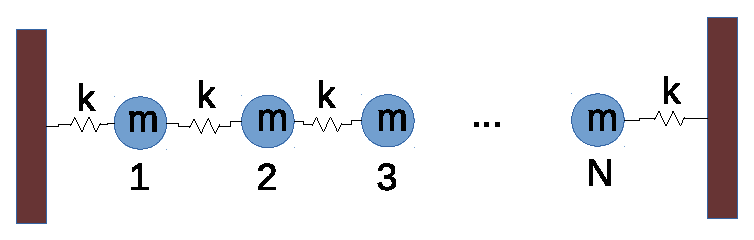
\includegraphics{p1}
\\
We compute the dispersion relation, which is the mode-dependence of the frequency $\omega_{\hat{m}}=\omega_0\times2\sin{\frac{\hat{m}}{N+1}\frac{\pi}{2}}$.
\\ \\
The expected value of the energy in mode j is:
\begin{gather}
 <E_j>=(\bar{n}(j)+\frac{1}{2})\hbar \omega_j,\ \bar{n}=\frac{1}{e^{\beta\hbar \omega_j}-1}
\end{gather}
The total mean thermal energy can be written as a sum of the individual mode terms.
\begin{gather}
 <E>=\sum_j(\bar{n}(j)+\frac{1}{2})\hbar \omega_j
\end{gather}
We can clear separate the $\bar{n}(j)$ and $\frac{1}{2}$ terms of the sum.
\begin{gather}
 <E>=\sum_j\bar{n}(j)\hbar \omega_j+\sum_j \frac{1}{2}\hbar \omega_j
\end{gather}
The left term depends on the temperature ($\beta=\frac{1}{kT}$), the right term is temperature independent.\\ \\
We expand the left sum:
\begin{gather}
 \sum_j\bar{n}(j)\hbar \omega_j=\sum_j \frac{\hbar \omega_j}{e^{\frac{\hbar \omega_j}{kT}}-1}
\end{gather}


\end{document}
